\documentclass[a4paper]{book}
% chktex-file 
% chktex-file 3
\usepackage{geometry}
% make full use of A4 papers
\geometry{margin=1.5cm, vmargin={0pt,1cm}}
\setlength{\topmargin}{-1cm}
\setlength{\paperheight}{29.7cm}
\setlength{\textheight}{25.1cm}

% auto adjust the marginals
\usepackage{marginfix}

\usepackage{amsfonts}
\usepackage{amsmath}
\usepackage{amssymb}
\usepackage{amsthm}
% \usepackage{CJKutf8}   % for Chinese characters
\usepackage{ctex}
\usepackage{enumerate}
\usepackage{graphicx}  % for figures
\usepackage{layout}
\usepackage{multicol}  % multiple columns to reduce number of pages
\usepackage{mathrsfs}
\usepackage{fancyhdr}
\usepackage{subfigure}
\usepackage{tcolorbox}
\usepackage{tikz-cd}
\usepackage{listings}
\usepackage{xcolor} %代码高亮
\usepackage{braket}
\usepackage{graphicx}
\usepackage{subfigure}
% ------------------
% common commands %
% ------------------
% differentiation
\newcommand{\gen}[1]{\left\langle#1 \right\rangle}
\newcommand{\dif}{\mathrm{d}}
\newcommand{\difPx}[1]{\frac{\partial#1}{\partial x}}
\newcommand{\difPy}[1]{\frac{\partial#1}{\partial y}}
\newcommand{\Dim}{\mathrm{D}}
\newcommand{\avg}[1]{\left\langle#1 \right\rangle}
\newcommand{\sgn}{\mathrm{sgn}}
\newcommand{\Span}{\mathrm{span}}
\newcommand{\dom}{\mathrm{dom}}
\newcommand{\Arity}{\mathrm{arity}}
\newcommand{\Int}{\mathrm{Int}}
\newcommand{\Ext}{\mathrm{Ext}}
\newcommand{\Cl}{\mathrm{Cl}}
\newcommand{\Fr}{\mathrm{Fr}}
% group is generated by
\newcommand{\grb}[1]{\left\langle#1 \right\rangle}
% rank
\newcommand{\rank}{\mathrm{rank}}
\newcommand{\Iden}{\mathrm{Id}}

% this environment is for solutions of examples and exercises
\newenvironment{solution}%
{\noindent\textbf{Solution.}}%
{\qedhere}
% the following command is for disabling environments
% so that their contents do not show up in the pdf.
\makeatletter
\newcommand{\voidenvironment}[1]{%
  \expandafter\providecommand\csname env@#1@save@env\endcsname{}%
  \expandafter\providecommand\csname env@#1@process\endcsname{}%
  \@ifundefined{#1}{}{\RenewEnviron{#1}{}}%
}
\makeatother

% ---------------------------------------------
% commands specifically for complex analysis %
% ---------------------------------------------
% complex conjugate
\newcommand{\ccg}[1]{\overline{#1}}
% the imaginary unit
\newcommand{\ii}{\mathbf{i}}
% \newcommand{\ii}{\boldsymbol{i}}
% the real part
\newcommand{\Rez}{\mathrm{Re}\,}
% the imaginary part
\newcommand{\Imz}{\mathrm{Im}\,}
% punctured complex plane
\newcommand{\pcp}{\mathbb{C}^{\bullet}}
% the principle branch of the logarithm
\newcommand{\Log}{\mathrm{Log}}
% the principle value of a nonzero complex number
\newcommand{\Arg}{\mathrm{Arg}}
\newcommand{\Null}{\mathrm{null}}
\newcommand{\Range}{\mathrm{range}}
\newcommand{\Ker}{\mathrm{ker}}
\newcommand{\Iso}{\mathrm{Iso}}
\newcommand{\Aut}{\mathrm{Aut}}
\newcommand{\ord}{\mathrm{ord}}
\newcommand{\Res}{\mathrm{Res}}
% \newcommand{\GL2R}{\mathrm{GL}(2,\mathbb{R})}
\newcommand{\GL}{\mathrm{GL}}
\newcommand{\SL}{\mathrm{SL}}
\newcommand{\Dist}[2]{\left|{#1}-{#2}\right|}

\newcommand\tbbint{{-\mkern-16mu\int}}
\newcommand\tbint{{\mathchar'26 -\mkern-14mu\int}}
\newcommand\dbbint{{-\mkern-20mu\int}}
\newcommand\dbint{{\mathchar'26 -\mkern-26mu\int}}
\newcommand\bint{
  {\mathchoice{\dbint}{\tbint}{\tbint}{\tbint}}
}
\newcommand\bbint{
  {\mathchoice{\dbbint}{\tbbint}{\tbbint}{\tbbint}}
}





% ----------------------------------------
% theorem and theorem-like environments %
% ----------------------------------------
\numberwithin{equation}{chapter}
\theoremstyle{definition}

\newtheorem{thm}{Theorem}[chapter]
\newtheorem{axm}[thm]{Axiom}
\newtheorem{alg}[thm]{Algorithm}
\newtheorem{asm}[thm]{Assumption}
\newtheorem{defn}[thm]{Definition}
\newtheorem{prop}[thm]{Proposition}
\newtheorem{rul}[thm]{Rule}
\newtheorem{coro}[thm]{Corollary}
\newtheorem{lem}[thm]{Lemma}
\newtheorem{exm}{Example}[chapter]
\newtheorem{rem}{Remark}[chapter]
\newtheorem{exc}[exm]{Exercise}
\newtheorem{frm}[thm]{Formula}
\newtheorem{ntn}{Notation}

% for complying with the convention in the textbook
\newtheorem{rmk}[thm]{Remark}


% \lstset{
%	backgroundcolor=\color{red!50!green!50!blue!50},%代码块背景色为浅灰色
%	rulesepcolor= \color{gray}, %代码块边框颜色
%	breaklines=true,  %代码过长则换行
%	numbers=left, %行号在左侧显示
%	numberstyle= \small,%行号字体
%	keywordstyle= \color{blue},%关键字颜色
%	commentstyle=\color{gray}, %注释颜色
%	frame=shadowbox%用方框框住代码块
% }
\lstset{
  columns=fixed,
  numbers=left,                                        % 在左侧显示行号
  numberstyle=\tiny\color{gray},                       % 设定行号格式
  frame=none,                                          % 不显示背景边框
  backgroundcolor=\color[RGB]{245,245,244},            % 设定背景颜色
  keywordstyle=\color[RGB]{40,40,255},                 % 设定关键字颜色
  numberstyle=\footnotesize\color{darkgray},
  commentstyle=\it\color[RGB]{0,96,96},                % 设置代码注释的格式
  stringstyle=\rmfamily\slshape\color[RGB]{128,0,0},   % 设置字符串格式
  showstringspaces=false,                              % 不显示字符串中的空格
  language=c++,                                        % 设置语言
}

% ----------------------
% the end of preamble %
% ----------------------

\begin{document}
\pagestyle{empty}
\pagenumbering{roman}
% 
% \tableofcontents
% \clearpage

% \pagestyle{fancy}
% \fancyhead{}
% \lhead{Qinghai Zhang}
% \chead{Notes on Algebraic Topology}
% \rhead{Fall 2018}


\setcounter{chapter}{0}
\pagenumbering{arabic}
% \setcounter{page}{0}

% --------------------------------------------------------
% uncomment the following to remove these environments
% to generate handouts for students.
% --------------------------------------------------------
% \begingroup
% \voidenvironment{rem}%
% \voidenvironment{proof}%
% \voidenvironment{solution}%


% each chapter is factored into a separate file.

\chapter{Homework 12235005 谭焱}

\section{1.10.2}
\exc Derive the stability condition for the Euler 
approximation to $u_t = u_{xx} +
u_{yy} + u_{zz}$ . Prove that the DuFort-Frankel 
method is unconditionally stable for the same equation.

\begin{solution}
  \begin{itemize}
    \item 
  Euler approximation is 
  \[v_j^{n+1} = (I + k(D_{+x}D_{-x}+ D_{+y}D_{-y}+
  D_{+y}D_{-y}) )v_j^n.\]
  By already know $kD_{+}D_{-} e^{i\omega x_j} = -4\sigma \sin^2
   \frac{\xi }{2} e^{i\omega x_j} $,
   where $\sigma = k/h^2, \xi = \omega h$. Get the symbol 
   \[\hat{Q} = 1 - 4\sigma ( \sin^2\frac{\xi_x }{2} +
   \sin^2\frac{\xi_y }{2} + sin^2\frac{\xi_z }{2}).\]
   
   Stable condition $| \hat{Q}| < 1$ imply
     \[\frac{k}{h^2} = \sigma < \frac{1}{6}.\]

\item DuFort-Frankel method is 
 \[v_j^{n+1} = \frac{1}{1 + 6\sigma}(
   2\sigma(D_{+x} + D_{-x} + D_{+y} + D_{-y}+
   D_{+y} + D_{-y}) v_j^{n} + (1 - 6\sigma )v_j^{n-1}).\]

   Now the characteristic equation is
   \[z^2 - \frac{4\sigma}{1 + 6\sigma}(\cos \xi_1 
   + \cos \xi_2 + \cos \xi_3)z - \frac{1 - 6\sigma}{1 + 6\sigma} = 0.\]
   that is,
   \[z_{1, 2} = \frac{2\sigma}{1 + 6\sigma}(\sum \cos\xi)
   \pm \frac{1}{1 + 6\sigma}\sqrt{A},\]
   where $A = 4\sigma^2(\sum \cos \xi)^2  + 1 - 36\sigma^2$.
    If $|A| \geq 0$, then $|A| \le 1$, and 
    \[|z_{1, 2}| \le \frac{6 \sigma}{1 + 6\sigma} + \frac{1}{1 + 6\sigma} = 1.\]

    If $|A| \le 0$, then we write 
    \[z_{1, 2} = \frac{1}{1 + 6\sigma}(2\sigma(
      \sum \cos \xi
    ) \pm i \sqrt{-A}).\]

    and get 
    \[|z_{1, 2}| = \frac{36 \sigma^2 - 1 }{(1 + 6 \sigma)^2}
    = \frac{6\sigma -1}{6\sigma +1} \le 1.\]
    That means DuFort-Frankel method is unconditionally stable.
    \end{itemize}
\end{solution}



\section{Program}
运行 matlab/leapFrogPeriod.m 复现程序结果如下

\begin{figure}[!h]
  \caption{initial function 1}
  \centering
  \subfigure[$Q_2$]{
  \begin{minipage}[t]{0.3\linewidth}
  \centering
  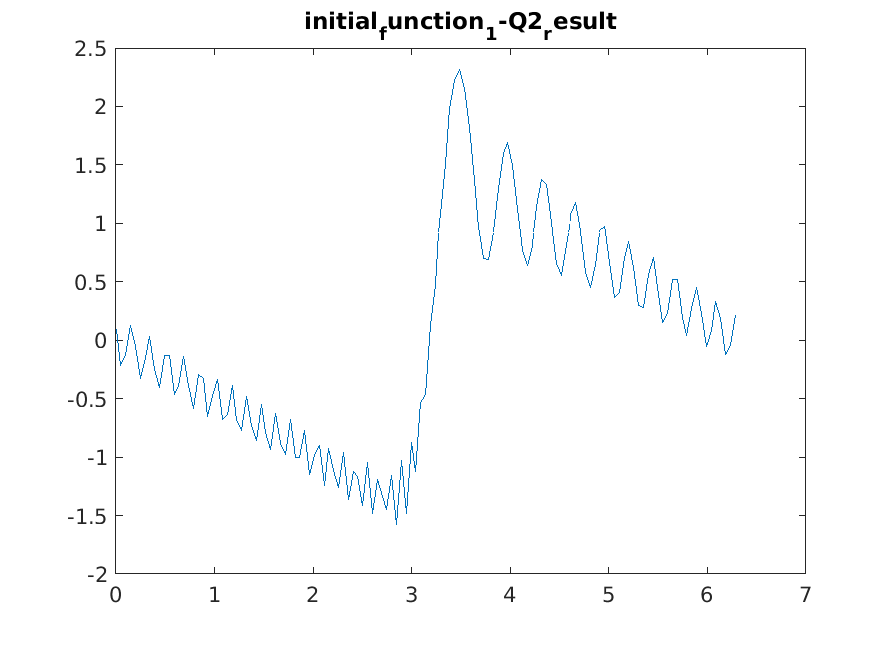
\includegraphics[height=2in, width=2in]{fig/initial_function_1-Q2_result.png}
  %\caption{fig1}
  \end{minipage}%
  }%
  \subfigure[$Q_4$]{
  \begin{minipage}[t]{0.3\linewidth}
  \centering
  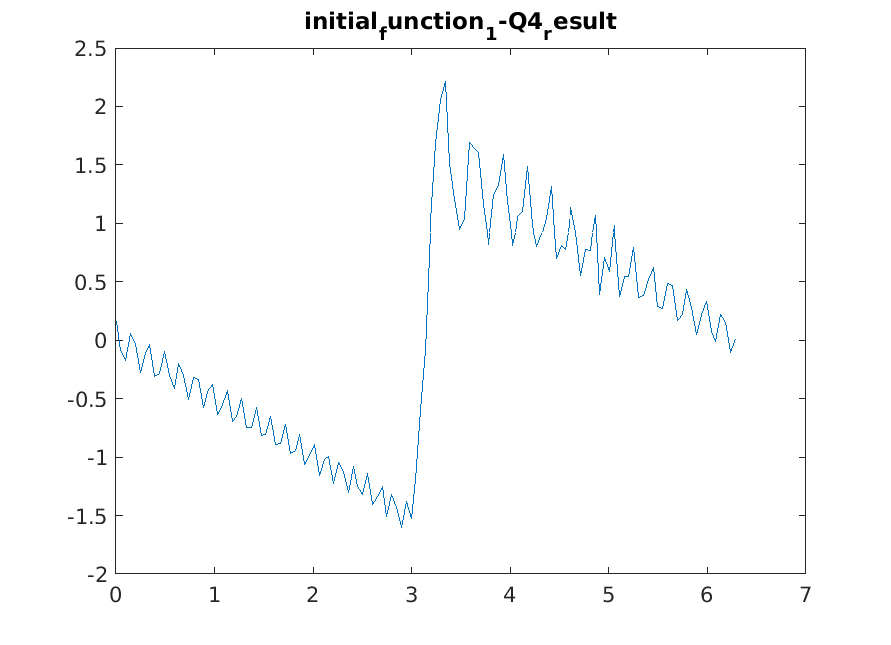
\includegraphics[height=2in, width=2in]{fig/initial_function_1-Q4_result.png}
  %\caption{fig1}
  \end{minipage}%
  }%
  \subfigure[$Q_6$]{
  \begin{minipage}[t]{0.3\linewidth}
  \centering
  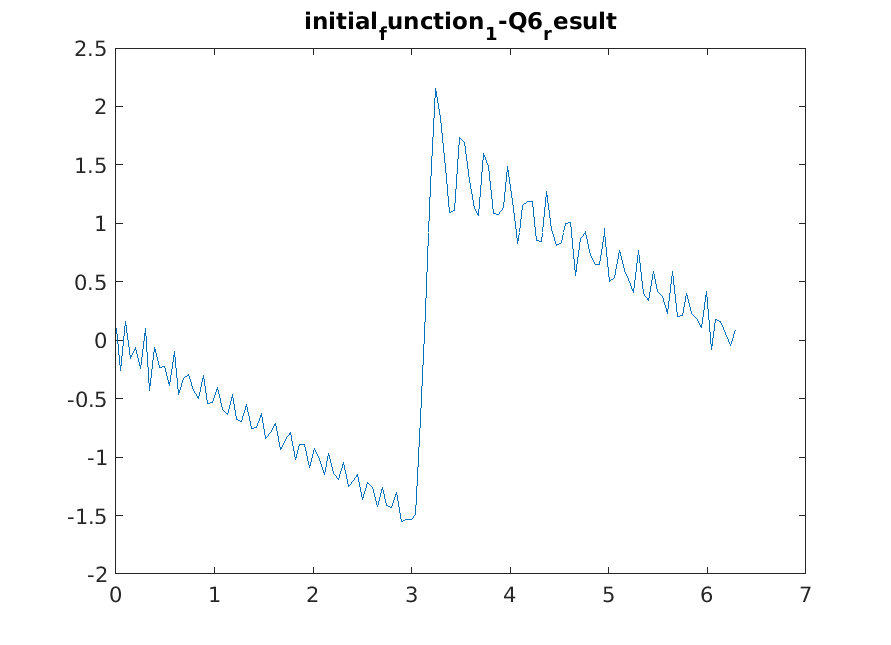
\includegraphics[height=2in, width=2in]{fig/initial_function_1-Q6_result.png}
  %\caption{fig1}
  \end{minipage}%
  }%
  
\end{figure}

\begin{figure}[!h]
  \caption{initial function 2}
  \centering
  \subfigure[$Q_2$]{
  \begin{minipage}[t]{0.3\linewidth}
  \centering
  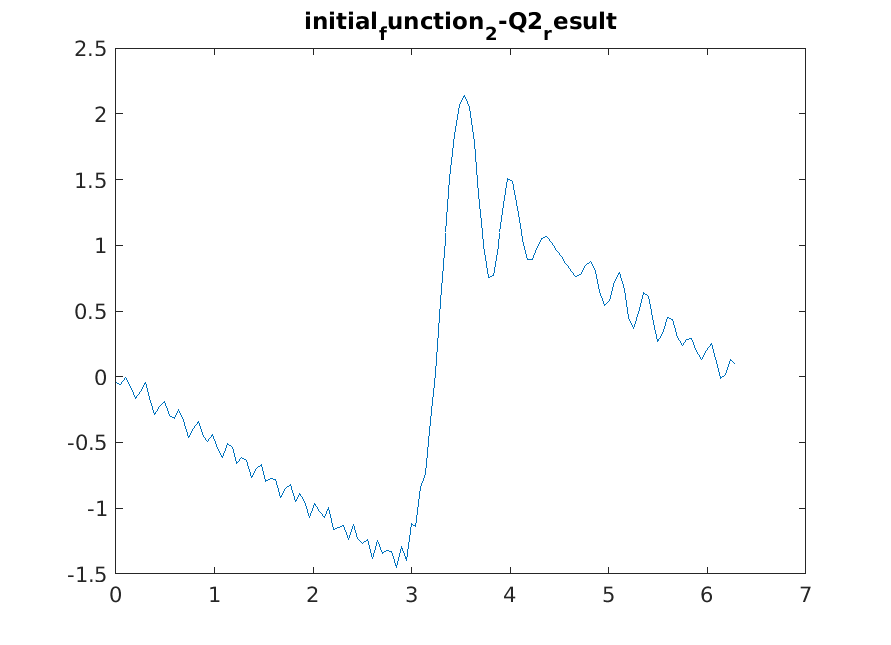
\includegraphics[height=2in, width=2in]{fig/initial_function_2-Q2_result.png}
  %\caption{fig1}
  \end{minipage}%
  }%
  \subfigure[$Q_4$]{
  \begin{minipage}[t]{0.3\linewidth}
  \centering
  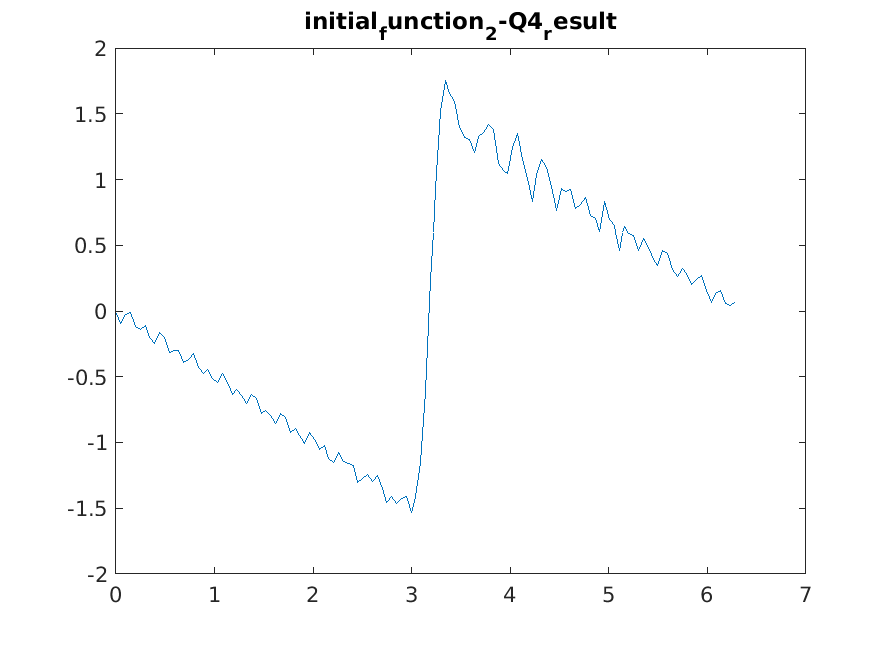
\includegraphics[height=2in, width=2in]{fig/initial_function_2-Q4_result.png}
  %\caption{fig1}
  \end{minipage}%
  }%
  \subfigure[$Q_6$]{
  \begin{minipage}[t]{0.3\linewidth}
  \centering
  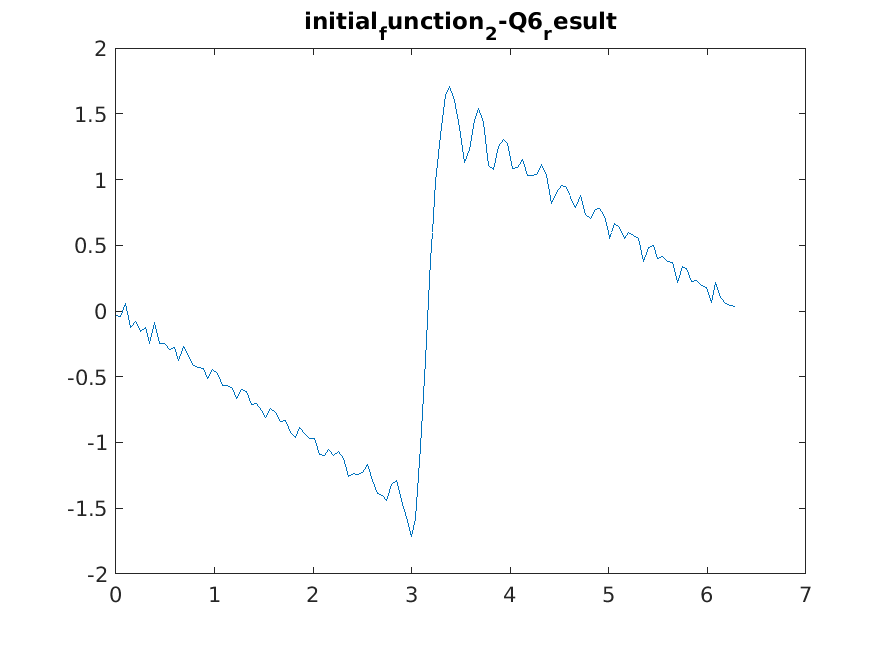
\includegraphics[height=2in, width=2in]{fig/initial_function_2-Q6_result.png}
  %\caption{fig1}
  \end{minipage}%
  }%
  
\end{figure}

\begin{figure}[!h]
  \caption{initial function 3}
  \centering
  \subfigure[$Q_2$]{
  \begin{minipage}[t]{0.3\linewidth}
  \centering
  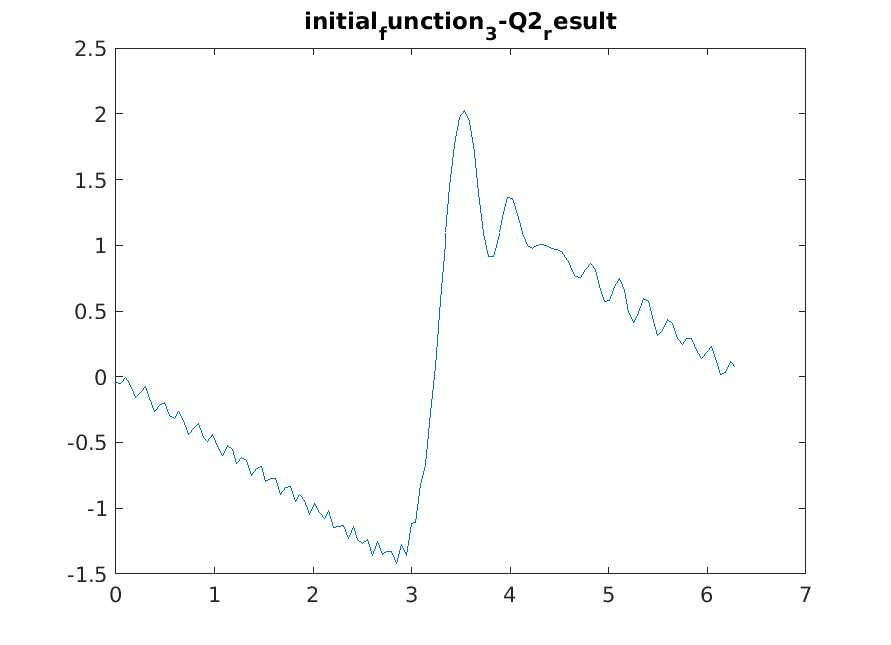
\includegraphics[height=2in, width=2in]{fig/initial_function_3-Q2_result.png}
  %\caption{fig1}
  \end{minipage}%
  }%
  \subfigure[$Q_4$]{
  \begin{minipage}[t]{0.3\linewidth}
  \centering
  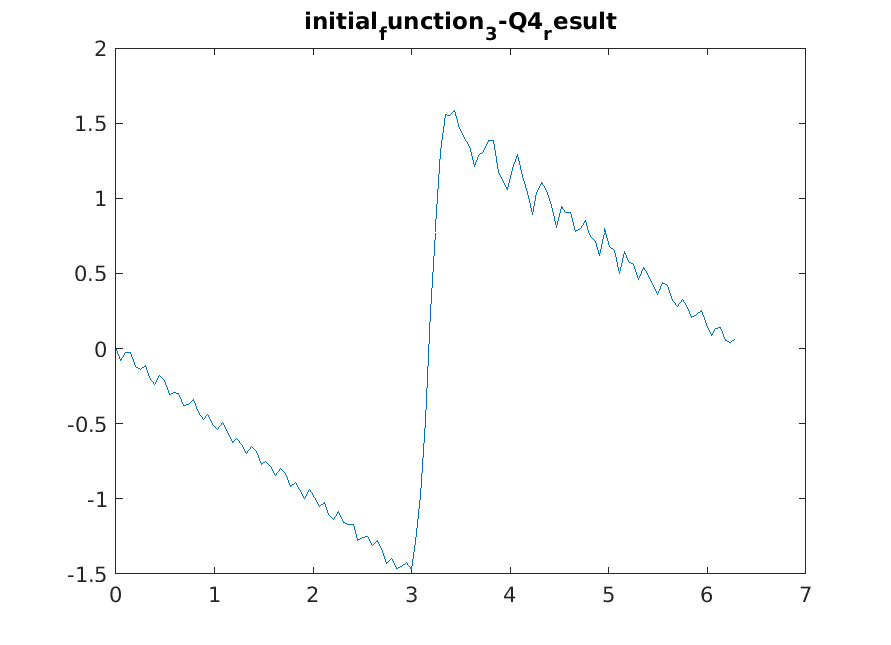
\includegraphics[height=2in, width=2in]{fig/initial_function_3-Q4_result.png}
  %\caption{fig1}
  \end{minipage}%
  }%
  \subfigure[$Q_6$]{
  \begin{minipage}[t]{0.3\linewidth}
  \centering
  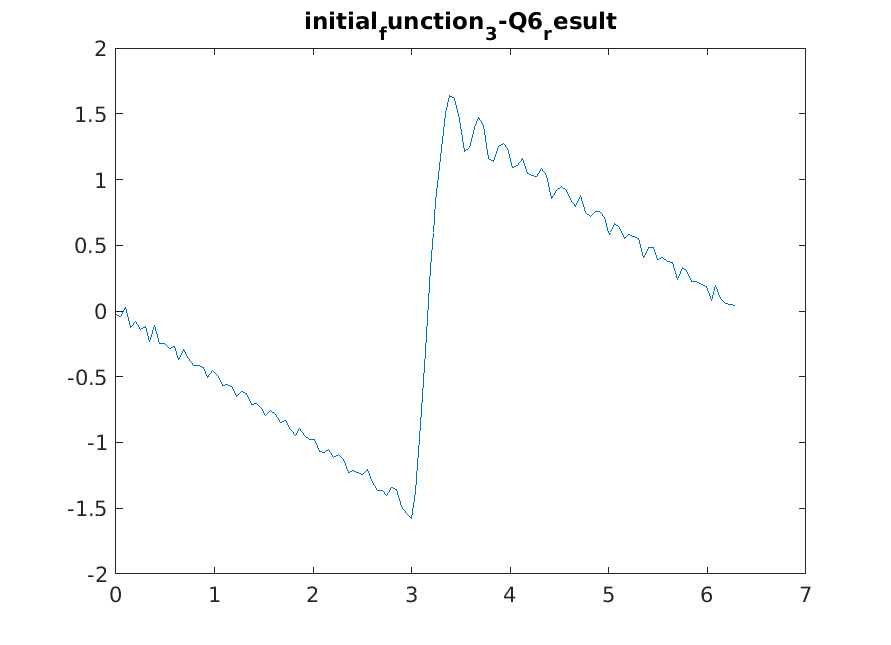
\includegraphics[height=2in, width=2in]{fig/initial_function_3-Q6_result.png}
  %\caption{fig1}
  \end{minipage}%
  }%
  
\end{figure}

\end{document}